\chapter{Design}
\label{cha:Design}
\newtext{All new text}
For the initial development of the simulator I focused on creating a working prototype for S2S merges. The S2S merge is one of the most simple merge scenarios that an autonomous vehicle might encounter. The designs here can then be expanded at a later date to include some of the other scenarios in \ref{sec:Merge Types}.

\section{Map}
\label{sec:Map}
In order to build the map using the user's parameters we will need to calculate the relative positions of the lane entrances and exits as well as the locations of the data collection lines and spawn points. A more detailed analysis of the mathematics used to calculate these positions can be found in Appendix \ref{sec:S2SMapCalculations}.

\subsection{Target Lane Coordinates}
\label{subsec:Target Lane Coordinates}
The target lane entrance will have a Y-coordinate equal to half of the lane width. In fact, every coordinate that target vehicles travel on will have a Y-coordinate equal to half the lane width. The entrance's X-coordinate will depend on whether the target lane, plus the merge zone length, is longer than the base width of the merging lane, that is, the horizontal distance the merging lane covers. You can see this distance indicated in Figure \ref{fig:baseWidth}.

\begin{figure}[htb]
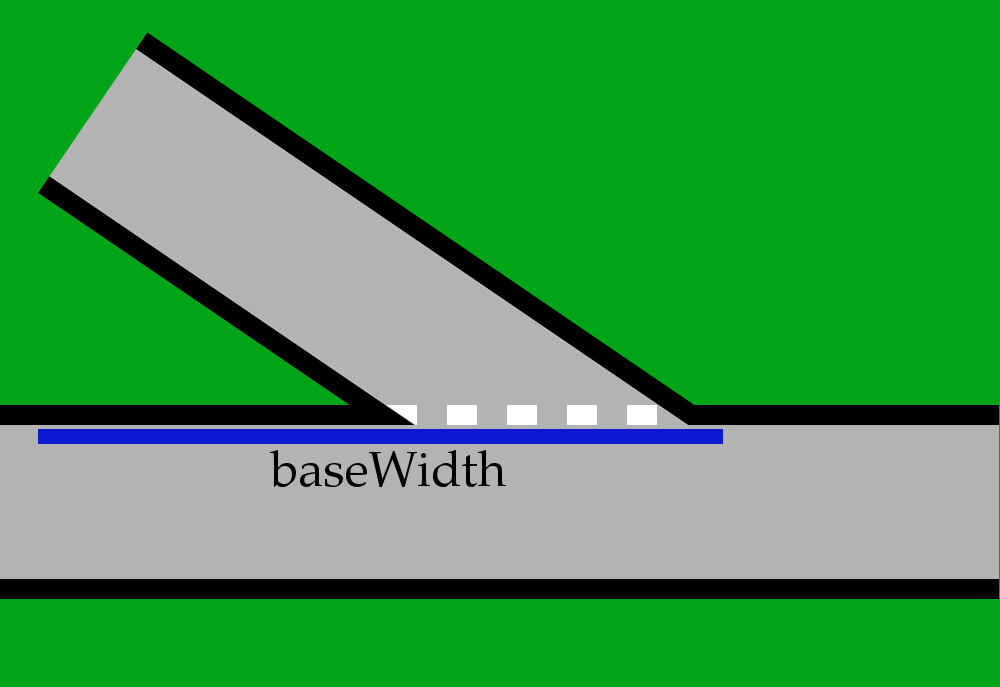
\includegraphics[width=\textwidth]{designNotes/baseWidth.png}
\caption{A diagram indicating the base width of the merging lane.}
\label{fig:baseWidth}
\end{figure}

If the target lane is longer then the entrance X-coordinate will be $0$. If not then we have to do further calculations. The total width of the simulation is given by equation \ref{targetLongerWidth} if the target lane has $x=0$ and equation \ref{mergeLongerWidth} if not.

\begin{multline}\label{targetLongerWidth}
width = \\
targetLeadInDistance + mergeZoneWidth + targetLeadOutDistance
\end{multline}

\begin{multline}\label{mergeLongerWidth}
width = mergeBaseWidth + targetLeadOutDistance
\end{multline}

So we can use equation \ref{targetLongerWidth} to calculate the target lane's entrance X-coordinate.

\begin{multline}\label{targetLaneStartX}
targetLaneStartX = width - \\
(targetLeadInDistance + mergeZoneWidth + targetLeadOutDistance)
\end{multline}

The target lane exit coordinates can be calculated similarly. The X-coordinate will be equal to the width of the simulator. With these coordinates calculated the simulator can place data collection lines and create spawn points for the target vehicles.

Finally the X-coordinate indicating the entrance to the merge zone for target vehicles is given by equation \ref{targetLaneZoneEntranceX}. The exit X-coordinate is given by equation \ref{targetLaneZoneExitX}.

\begin{multline}\label{targetLaneZoneEntranceX}
targetLaneZoneEntranceX = width - \\
(mergeZoneWidth + targetLeadOutDistance)
\end{multline}

\begin{multline}\label{targetLaneZoneExitX}
targetLaneZoneExitX = width - targetLeadOutDistance
\end{multline}

\subsection{Merging Lane Coordinates}
\label{subsec:Merging Lane Coordinates}
The merging lane entrance coordinates are more difficult to calculate. To get the X-coordinate we can calculate an x-adjustment from the far edge of the lane to the centre, as shown in Figure \ref{fig:adjustments}.

\begin{figure}[htb]
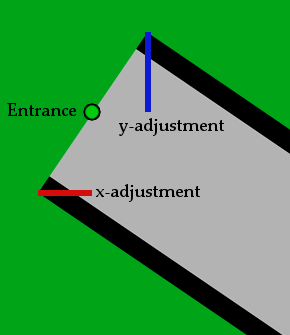
\includegraphics[width=\textwidth]{designNotes/adjustments.png}
\caption{A diagram indicating the x and y adjustments for the merging lane.}
\label{fig:adjustments}
\end{figure}

To get the Y-coordinate we can calculate the distance the coordinate is above the target lane, and then add the width of the target lane to that. We can also use this length to calculate the height of the whole simulator. However, to do that we will also need to add a y-adjustment, also shown in Figure \ref{fig:adjustments}.

Merge vehicles will exit the merge zone in the same place as target vehicles (equation \ref{targetLaneZoneExitX}), however, they will enter the merge zone at the top. The Y-coordinate of this point is equal to the width of the target lane. The X-coordinate is given by equation \ref{mergeLaneZoneEntranceX}.

\begin{multline}\label{mergeLaneZoneEntranceX}
mergeLaneZoneEntranceX = width - \\
targetLeadOutDistance - \frac{mergeZoneWidth}{2}
\end{multline}

After the merge vehicles enter the merge zone they will deviate from the lane, however the merge lane centre does continue until it reaches the centre of the target lane. We know this centre has a Y-coordinate equal to half of the lane width. The X-coordinate is more difficult to calculate. We need to find another X-adjustment, denoted as centreXAdjustment, along the target lane centre line. We can then use equation \ref{connectionPointX} to find the X-coordinate. Figure 

\begin{multline}\label{connectionPointX}
connectionPointX = width - \\
targetLeadOutDistance - \frac{mergeZoneWidth}{2} + centreXAdjustment
\end{multline}

\begin{figure}[htb]
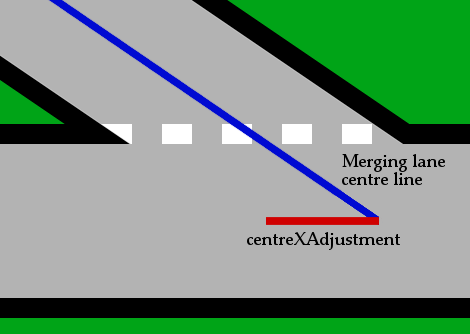
\includegraphics[width=\textwidth]{designNotes/centreXAdjustment.png}
\caption{A diagram indicating the X-adjustment used to find the point at which the two lanes connect.}
\label{fig:centreXAdjustment}
\end{figure}.

\section{Intersection Management System}
\label{subsec:Intersection Management System}

\section{Decentralised Communication System}
\label{subsec:Decentralised Communication System}

\section{Measuring Success}
\label{subsec:Measuring Success}
